\documentclass[10pt]{article}
\usepackage[margin=0.9in]{geometry}
\usepackage[T1]{fontenc}
\usepackage{newtxtext,newtxmath}
\usepackage{cite}
\usepackage{amsmath}
\let\openbox\undefined
\usepackage{amsthm}
\usepackage{booktabs}
\usepackage{array}
\usepackage{multirow}
\usepackage{float}
\usepackage{microtype}
\usepackage{xcolor}
\usepackage{enumitem}
\usepackage{tikz}
\usetikzlibrary{arrows.meta,positioning,fit,backgrounds,shapes.geometric,calc,decorations.pathreplacing}
\usepackage{caption}
\usepackage{titlesec}
\usepackage{fancyhdr}
\usepackage{url}
\usepackage{algorithm}
\usepackage{algpseudocode}
\usepackage[hidelinks]{hyperref}
\hypersetup{
  pdftitle={StanceJEV: Typed Probabilistic Stance Detection with Consistency-Verified Decisions},
  pdfauthor={Hazel Bloomer},
  pdfsubject={Zero-shot stance detection with a typed DecisionSOP terminal contract},
  pdfkeywords={stance detection, typed decision systems, Jev, DecisionSOP, consistency verification, zero-shot}
}

\captionsetup{font=small,labelfont=bf,labelsep=period,skip=5pt}
\titleformat{\section}{\normalfont\large\bfseries}{\thesection}{0.7em}{}
\titleformat{\subsection}{\normalfont\bfseries}{\thesubsection}{0.6em}{}
\titleformat{\subsubsection}{\normalfont\itshape}{\thesubsubsection}{0.5em}{}
\titlespacing*{\section}{0pt}{13pt plus 2pt minus 2pt}{6pt}
\titlespacing*{\subsection}{0pt}{9pt plus 1pt minus 1pt}{4pt}
\titlespacing*{\subsubsection}{0pt}{7pt plus 1pt minus 1pt}{3pt}
\setlist[itemize]{leftmargin=1.15em,itemsep=2pt,topsep=3pt,parsep=0pt}
\setlist[enumerate]{leftmargin=1.25em,itemsep=2pt,topsep=3pt,parsep=0pt}
\setlength{\abovedisplayskip}{6pt}
\setlength{\belowdisplayskip}{6pt}
\setlength{\abovedisplayshortskip}{3pt}
\setlength{\belowdisplayshortskip}{3pt}
\raggedbottom

\pagestyle{fancy}
\fancyhf{}
\fancyhead[L]{\footnotesize\itshape Hazel Bloomer}
\fancyhead[R]{\footnotesize\itshape StanceJEV}
\renewcommand{\headrulewidth}{0.3pt}
\fancyfoot[C]{\footnotesize\thepage}

\theoremstyle{definition}
\newtheorem{definition}{Definition}
\newtheorem{remark}{Remark}

\begin{document}

\title{\vspace{-2.2em}\bfseries\Large StanceJEV: Typed Probabilistic Stance Detection\\[2pt]
with Consistency-Verified Decisions}
\author{\normalsize Hazel Bloomer\\[2pt]
{\small Independent Researcher}\\[1pt]
{\small\texttt{floanpaarnatl@outlook.com}}}
\date{}
\maketitle
\vspace{-1.1em}

\begin{abstract}
\noindent Zero-shot stance detection underpins social monitoring and agent tooling, yet deployed consumers
require machine-consumable labels in $\{\texttt{Favor},\texttt{Against},\texttt{None}\}$ rather than
free-form text that must still be parsed and re-validated after every call.
Recent LLM and small--large collaborative pipelines improve predictive accuracy and query cost, but leave the
\emph{terminal decision interface} free-form even though stance labels already form a closed action set.
We formulate zero-shot stance as a \emph{typed probabilistic choice} over that set, place CoVer-style
context reconstruction, batch reasoning, and a consistency gate \emph{before} emission, and terminate in a
Jev~/~DecisionSOP contract that returns $p(y)$ with an auditable trace.
The resulting system, \textbf{StanceJEV}, yields schema-valid labels by construction.
On SemEval-2016 Task~A ($n{=}1{,}249$) it reaches $F_{\mathrm{AVG}}{=}0.785$ at $Q_{\mathrm{AVG}}{=}2.0$
with $100\%$ schema-valid typed labels; on VAST zero-shot ($n{=}1{,}460$) it reaches
$F_{\mathrm{macro3}}{=}0.833$ under the same configuration.
Analysis of typed peak probability shows that accuracy rises monotonically across max-$p$ bins, while the
consistency score $\kappa$ characterizes agreement between batch likelihoods and the verifier rather than
serving as a calibrated correctness proxy under a single-round budget.
These results indicate that evaluating only free-form accuracy leaves the decision interface unsolved:
stance monitoring needs a typed terminal contract.
\end{abstract}

\vspace{0.35em}
\noindent\textbf{Keywords:} stance detection; typed decision systems; Jev; consistency verification;
DecisionSOP; zero-shot evaluation; monitoring interfaces

%==============================================================================
\section{Introduction}
\label{sec:intro}
%==============================================================================

Stance detection maps a text and a target to a label in
$\mathcal{Y}=\{\texttt{Favor},\texttt{Against},\texttt{None}\}$
\cite{mohammad2016semeval,allaway2020vast}.
The scientific and engineering setting that motivates this paper is not offline leaderboard scoring alone.
In production monitoring---topic dashboards, alert triage, content routing, and tool-using agents---the
downstream consumer is \emph{code}.
That consumer needs a closed label, a probability vector, and a trace that can be stored, filtered, and
audited.
It does not need a generative paragraph that must be regularized, parsed, and schema-checked after every
model call.
Consider three concrete consumers.
A streaming monitor must fan predictions into topic counters without a human in the loop; a brittle parse that
maps ``leans against'' to an unknown string breaks the counter.
An alert policy must threshold on probability mass (e.g., act only when $\max_y p(y)$ exceeds a cut-off); free-form
text does not expose that mass unless a second model or heuristic invents it.
An agent tool must return a JSON-shaped action that downstream planners can branch on; schema violations become
tool errors rather than soft NLP disagreements.
Across these settings the scientific question is not only whether a model can \emph{say} the right stance, but
whether the system can \emph{emit} a closed decision that other software can trust.

Existing approaches address the accuracy and cost sides of this problem with increasing sophistication.
Supervised and contrastive SLMs transfer stance cues across targets
\cite{liang2022jointcl,liu2019roberta}.
LLM reasoners raise zero-shot coverage with demonstrations and chain-of-thought
\cite{zhang2022chatgptstance,zhang2023cotstance,wei2022cot}.
Collaborative systems such as CoVer combine LLM batch reasoning with SLM consistency verification, reducing
query cost while improving accuracy \cite{yan2025cover}.
Across these lines the \emph{terminal} output remains free-form or loosely structured text.
Accuracy and cost improve; the decision interface does not.
Parse failures, near-label paraphrases, and missing probability mass are pushed into evaluation scripts and
deployment glue---outside the model contract that the literature reports as ``stance accuracy.''

We argue that the underlying issue is contractual rather than purely representational.
Stance labels already constitute a closed action set.
Treating the task as open-ended generation therefore solves a harder problem than the monitoring product
requires, then relocates schema fidelity to post-processing.
Typed decision interfaces reverse that order: a Jev \texttt{choice} over $\mathcal{Y}$ returns
$p(y\mid s,\mathcal{Y})$ with the selected label inside $\mathcal{Y}$ by construction
\cite{typesafe2026systemone,typesafe2026jev,openrouter2026jev}, and jevtree packages the call as an
auditable DecisionSOP \cite{jevtree2026}.
The natural place for CoVer-style reconstruction, batch reasoning, and consistency verification is
\emph{before} that typed emission, so that low-consistency items are flagged in the state rather than silently
trusted as fluent free-form text.

This observation yields StanceJEV: a zero-shot stance path whose contribution is the reformulation of stance
as a typed probabilistic decision with a consistency gate on the path to emission.
Empirically, under a fixed remote query budget $Q_{\mathrm{AVG}}{=}2.0$ (one batch-reasoning call and one typed
decision call per item; local verifier~/~keep-all CR excluded), the path reaches $F_{\mathrm{AVG}}{=}0.785$ on SemEval-2016 Task~A
($n{=}1{,}249$) and $F_{\mathrm{macro3}}{=}0.833$ on VAST zero-shot ($n{=}1{,}460$), with $100\%$
schema-valid labels on both suites.
Security analyses of the same typed interface study how untrusted content shifts probabilities inside a closed
action set \cite{wu2026decisionhijacking}; that line is complementary to the monitoring path developed here.

\paragraph{Contributions.}
\begin{itemize}
\item \textbf{Formulation.}
  We identify the unresolved gap in zero-shot stance as the terminal decision interface: free-form accuracy
  leaves schema fidelity and consumability outside the evaluation contract, even though $\mathcal{Y}$ is
  already a closed action set.
\item \textbf{Method.}
  We formulate stance as a typed probabilistic choice over $\mathcal{Y}$, place a CoVer-style consistency
  path (context reconstruction, batch reasoning, consistency gate) before emission, and terminate in a
  DecisionSOP record that carries both $p(y)$ and the admission signal $\kappa$.
\item \textbf{Evidence.}
  On SemEval-2016 Task~A and VAST zero-shot, the typed path delivers
  $F_{\mathrm{AVG}}{=}0.785$ and $F_{\mathrm{macro3}}{=}0.833$ at $Q_{\mathrm{AVG}}{=}2.0$ with universal
  schema validity; typed peak probability concentrates on correct items, while $\kappa$ reports
  batch--verifier agreement under a single-round budget.
\end{itemize}

Section~\ref{sec:related} situates the work against stance SLMs/LLMs, collaborative SLLM pipelines, and typed
decision systems.
Section~\ref{sec:method} develops the problem, principle, and design.
Sections~\ref{sec:setup}--\ref{sec:results} report protocol, main results, fidelity statistics, and analyses
computed from the typed prediction traces.
Section~\ref{sec:discussion} discusses implications for monitoring interfaces, relation to CoVer, and scope;
Section~\ref{sec:conclusion} concludes.

%==============================================================================
\section{Related Work}
\label{sec:related}
%==============================================================================

\subsection{Stance detection with SLMs and LLMs}
SemEval-2016 Task~6, VAST, and P-Stance establish the Favor~/~Against~/~None framing under in-target and
zero-shot splits \cite{mohammad2016semeval,allaway2020vast,li2021pstance}.
These benchmarks differ in target cardinality and domain: SemEval concentrates five campaign targets with
short tweets; VAST spans hundreds of topics with longer comments and an explicit zero-shot split; P-Stance
emphasizes political Twitter figures.
JointCL strengthens zero-shot transfer through contrastive topic--text learning \cite{liang2022jointcl}, and
encoder pretraining such as RoBERTa remains a common SLM backbone \cite{liu2019roberta}.

LLM pipelines explore demonstrations, chain-of-thought, logically consistent reasoning, multi-agent debate,
and counterfactual calibration
\cite{zhang2022chatgptstance,zhang2023cotstance,zhang2023lccot,lan2024cola,li2024factual,wei2022cot}.
These methods advance predictive quality and, in several cases, interpretability of intermediate explanations.
They do not redefine the terminal label as a typed choice: evaluation scripts still recover $\mathcal{Y}$ from
generated strings, and schema violations are handled outside the reported metric when they occur.
Even when few-shot demos constrain surface form, the contract remains generative: nothing in the model API
guarantees that every future call stays inside $\mathcal{Y}$ or returns a calibrated simplex over it.
The monitoring consumer---who must ingest every prediction---inherits that residual interface problem.
Bias-aware calibration further improves fairness of free-form or classifier scores \cite{li2024factual}, yet
still treats consumability as orthogonal to the reported stance metric.

\subsection{Collaborative small--large reasoning}
CoVer couples knowledge-aware context reconstruction, batch LLM reasoning, SLM explanation--label
verification, and weighted aggregation, reporting strong zero-shot accuracy at low query cost
\cite{yan2025cover}.
The collaboration answers a concrete deployment question: when is a single batch LLM call trustworthy enough
to accept, and when should the system re-query or aggregate?
Related retrieval and embedding components (e.g., multi-granularity embedders) support reconstruction of short
or knowledge-dependent inputs \cite{chen2024bgem3}.

StanceJEV retains that collaboration pattern as the path \emph{into} a typed endpoint.
The collaboration improves \emph{when} to trust a batch call; the typed choice fixes \emph{what} the system is
allowed to emit.
This separation matters for evaluation: accuracy and cost characterize the collaboration, while schema
validity and probability concentration characterize the terminal contract.
In other words, CoVer-style verification is necessary but not sufficient for monitoring deployment: a
high-$\kappa$ free-form string can still fail a downstream schema check, and a schema-valid enum without an
admission signal conceals whether the batch explanation was coherent.
The present work keeps both signals on one DecisionSOP surface.

\subsection{Typed decisions and agent security}
Jev and companion stacks make closed-set judgments consumable by ordinary code
\cite{typesafe2026systemone,typesafe2026jev,jevtree2026,jevforest2026}.
A typed \texttt{choice} returns a probability vector over a declared action set; jevtree exports DecisionSOP
specifications with feature trees and run-time traces.
Indirect injection and tool-agent benchmarks show that external text can redirect generative agents whose
action space is open-ended or tool-mediated
\cite{greshake2023indirect,zhan2024in,yi2025bipia,debenedetti2024agentdojo}.
Decision Hijacking studies probability shifts on Jev's closed action set under adversarial framing
\cite{wu2026decisionhijacking}.

Evaluation discipline further warns that surface success can diverge from grounded capability
\cite{souly2024strongreject,yan2025confusion}, with related analyses of metaphor framing, multimodal
entanglement, distributed synthesis, and search-augmented misuse
\cite{yan2025benign,yan2026red,yan2025poisonswarm,yan2026searchattack}.
These lines motivate inspectable typed contracts for agent and monitoring stacks; they do not themselves
supply a zero-shot stance monitoring path that binds CoVer-style verification to typed emission.
Budgeted feature acquisition in related typed stacks \cite{jevforest2026} further illustrates why closed
action sets are a natural fit for systems that must decide under cost constraints: the action is declared
before inference, and the trace records which evidence entered the decision.
Stance monitoring is an instance of that pattern where the action set is the stance label inventory itself.

\paragraph{Position.}
Prior work either optimizes free-form stance accuracy or studies typed decisions outside stance.
The unresolved gap is the interface between them: a zero-shot stance system whose terminal contract is a
typed probabilistic choice, with a consistency gate on the path to emission so that admission and label are
jointly auditable.

%==============================================================================
\section{Method}
\label{sec:method}
%==============================================================================

\subsection{Problem}
\label{sec:problem}
Given raw text $x_{\mathrm{raw}}$ and target $t$, predict $y\in\mathcal{Y}$ under zero-shot
\emph{inference}: the system sees no labeled examples of the evaluation targets at prediction time
\cite{allaway2020vast,yan2025cover}.
Let $\mathcal{D}_{\mathrm{test}}=\{(x_i,t_i,y_i)\}_{i=1}^{N}$ denote a held-out suite drawn from published
splits (VAST official $\texttt{seen?}{=}0$; SemEval-2016 Task~A official test).
No SemEval training data, in-context demonstrations from train, or target-specific supervision enter the
reported path.
The product constraint is stricter than open-ended generation: every prediction must be an element of
$\mathcal{Y}$, accompanied by a probability vector $p(\cdot)\in\Delta^{|\mathcal{Y}|-1}$ and a trace that a
monitoring stack can store and audit.

Primary accuracy metrics follow prior protocol: $F_{\mathrm{AVG}}$ (mean Favor~/~Against F1) on
SemEval-2016 Task~A, and three-label mean $F_{\mathrm{macro3}}$ on VAST
\cite{mohammad2016semeval,allaway2020vast,yan2025cover}.
We additionally report schema-valid rate, mean peak probability $\mathbb{E}[\max_y p(y)]$, and mean
consistency $\kappa$, so that interface fidelity is measured on the same surface as accuracy.

\subsection{Principle}
\label{sec:principle}
If $\mathcal{Y}$ is already the action set, the terminal step should be a \emph{choice} over $\mathcal{Y}$,
not a generation over an open vocabulary.
Accuracy-oriented modules then serve a different role: they construct and admit a state $s$ that is
trustworthy enough to present to that choice.
This separation---consistency before emission, typed choice at emission---is the design principle behind
StanceJEV.

Concretely, free-form termination fails in two distinct ways that a single accuracy number conflates:
(i)~the generated string may fall outside $\mathcal{Y}$ or require brittle parsing;
(ii)~a fluent string inside $\mathcal{Y}$ may rest on an inconsistent explanation.
Typed emission eliminates (i) by construction.
The consistency gate targets (ii) by scoring agreement between batch likelihoods and a verifier before the
typed call commits.

\subsection{Typed stance decision}
\begin{definition}[Typed stance decision]
\label{def:typedstance}
Let $A=\mathcal{Y}$ and let $s$ be a state carrying reconstructed text, target, and optional knowledge.
A \emph{typed stance decision} is a Jev \texttt{choice} that returns a probability vector
$p(a\mid s,A)$ and selected action $\hat{a}=\arg\max_a p(a\mid s,A)$, with $\hat{a}\in A$ by construction
\cite{typesafe2026jev,openrouter2026jev}.
\end{definition}
Labels outside $A$ cannot be emitted.
jevtree packages the call inside a DecisionSOP with optional feature tree and run-time traces
\cite{jevtree2026}.
In StanceJEV, $s$ is assembled by the path in Section~\ref{sec:path}; the typed call is never invoked on raw
$(x_{\mathrm{raw}},t)$ alone when reconstruction and batch evidence are available.

\subsection{Path to emission}
\label{sec:path}
Figure~\ref{fig:pipeline} summarizes the path.
Each stage answers a concrete failure mode of free-form termination.
Algorithm~\ref{alg:stancejev} states the control flow under a round budget $M$.

\paragraph{State.}
We write
\begin{equation}
s = \bigl(x_{\mathrm{rec}},\, t,\, e,\, P_{\mathrm{LLM}},\, \kappa\bigr),
\end{equation}
where $x_{\mathrm{rec}}$ is reconstructed text, $e$ is a batch explanation, $P_{\mathrm{LLM}}$ is a likelihood
vector on $\mathcal{Y}$, and $\kappa\in[0,1]$ is the consistency score defined below.

\paragraph{Context reconstruction (CR).}
Implicit and knowledge-dependent cues are a known failure mode for short social text
\cite{yan2025cover,chen2024bgem3}.
CR may attach linked knowledge when a knowledge field is present and, optionally, filter sentences by
stance entropy estimated with an embedder.
With sentence embedding $h_x$ and label prototypes $h_{s_y}$,
\begin{equation}
\label{eq:se}
\widehat{P}(y\mid x,t)=\frac{\exp(\mathrm{sim}(h_x,h_{s_y}))}{\sum_{y'}\exp(\mathrm{sim}(h_x,h_{s_{y'}}))},\quad
\mathrm{SE}_x=-\sum_{y}\widehat{P}(y\mid x,t)\log\widehat{P}(y\mid x,t).
\end{equation}
Sentences whose removal increases $\mathrm{SE}_x$ are treated as stance-informative and retained in
$x_{\mathrm{rec}}$.
Without recoverable context, the state $s$ presented to later stages omits cues that the typed choice cannot
invent from an open vocabulary.
The reported SJ-1 configuration uses keep-all reconstruction (no embedder call); Section~\ref{sec:setup}
records that choice.

\paragraph{Batch reasoning (BR).}
Remote query cost dominates zero-shot LLM deployment \cite{yan2025cover,wei2022cot}.
BR scores a batch $B=\{(x_i,t_i)\}$ in one shared remote call, returning explanation $e_i$ and likelihoods
$P_{\mathrm{LLM},i}\in\Delta^{2}$ for each item.
Batching amortizes prompt overhead; the explanations supply the evidence that the consistency gate will check.
We define $Q_{\mathrm{AVG}}$ as the mean number of \emph{remote} LLM~/~decision API calls per item.
Local modules (consistency verifier; keep-all CR with no embedder call) are not counted in that budget.
Under our evaluation protocol each accepted item uses one remote BR call and one remote typed call, so
$Q_{\mathrm{AVG}}{=}2.0$.

\paragraph{Consistency gate (CV).}
\begin{definition}[Consistency gate]
\label{def:gate}
A verifier (local lexicon heuristic in the reported system; optionally a remote SLM) scores $P_{\mathrm{SLM},i}=P(y\mid e_i,t_i)$ from the explanation--target pair.
Let $\mathrm{JS}$ denote Jensen--Shannon divergence on the stance simplex and let
$\mathrm{overlap}$ denote top-label agreement.
Define
\begin{equation}
\label{eq:kappa}
\kappa_i=(1-\lambda)\,(1-\mathrm{JS}(P_{\mathrm{LLM},i},P_{\mathrm{SLM},i}))
+\lambda\cdot\mathrm{overlap}(P_{\mathrm{LLM},i},P_{\mathrm{SLM},i}),
\end{equation}
with $\lambda{=}0.35$ following the CoVer-style mixture \cite{yan2025cover}.
The gate accepts $P_{\mathrm{LLM},i}$ when $\kappa_i\ge\tau$.
If $\kappa_i<\tau$ and fewer than $M$ rounds have been used, BR is re-invoked; if the score remains below
threshold after $M$ rounds, the system emits a consistency-weighted aggregate of stored likelihoods when
multiple rounds are available.
\end{definition}

When multiple rounds $\{(P^{(r)},\kappa^{(r)})\}_{r=1}^{R}$ are stored with $R>1$ and the final round remains
below threshold, the consistency-weighted aggregate is
\begin{equation}
\label{eq:agg}
P_{\mathrm{agg}}(y)=\frac{\sum_{r=1}^{R}\kappa^{(r)}P^{(r)}(y)}{\sum_{r=1}^{R}\kappa^{(r)}},\qquad y\in\mathcal{Y},
\end{equation}
which reduces to the single-round likelihood when $R{=}1$.

\begin{remark}[What the gate protects]
Without the gate, a single fluent but inconsistent batch explanation would pass unchanged into the typed
endpoint.
The gate therefore protects the quality of $s$, not the schema of $\hat{a}$---schema is already enforced by
Definition~\ref{def:typedstance}.
Under a single-round budget ($M{=}1$), $\kappa$ is recorded for every item and multi-round aggregation is
inactive; the typed emission still proceeds so that schema fidelity remains universal while $\kappa$ remains
an auditable admission signal.
\end{remark}

\paragraph{DecisionSOP record.}
Each item yields a record
\begin{equation}
\label{eq:sop}
\mathrm{SOP}_i=\bigl(\hat{y}_i,\,p_i(\cdot),\,\kappa_i,\,e_i,\,x_{\mathrm{rec},i},\,t_i,\,q_i\bigr),
\end{equation}
where $q_i$ is the per-item \emph{remote} query count (BR + typed call under our protocol).
Monitoring stacks can filter on $\hat{y}$, threshold on $\max_y p(y)$, audit $\kappa$, and store $e$ without
re-entering the generative model.
This is the operational meaning of ``typed probabilistic stance'': the scientific object is not only the
label, but the consumable record.

\paragraph{Typed emission.}
Accepted (or final-round) probabilities and the reconstructed state write into the Jev \texttt{choice} of
Definition~\ref{def:typedstance}.
Traces retain $e_i$, $\kappa_i$, $p(\cdot)$, and the accept~/~continue decision, forming the DecisionSOP
record for each item.
Placing typed emission \emph{after} CV is deliberate: the closed action set should reflect a state that has
already been checked for explanation--label coherence, rather than freezing an unchecked free-form string into
a label enum.

\begin{algorithm}[t]
\caption{StanceJEV path under round budget $M$}
\label{alg:stancejev}
\begin{algorithmic}[1]
\Require pair $(x_{\mathrm{raw}},t)$, threshold $\tau$, round budget $M\ge 1$
\State $x_{\mathrm{rec}}\gets\mathrm{CR}(x_{\mathrm{raw}},t)$
\State $\mathcal{R}\gets[\,]$ \Comment{ordered list of $(P_{\mathrm{LLM}},\kappa)$ rounds}
\For{$r=1$ to $M$}
  \State $(e,P_{\mathrm{LLM}})\gets\mathrm{BR}(x_{\mathrm{rec}},t)$ \Comment{batched across items}
  \State $\kappa\gets$ consistency$(P_{\mathrm{LLM}},e,t)$ via Eq.~\eqref{eq:kappa}
  \State append $(P_{\mathrm{LLM}},\kappa)$ to $\mathcal{R}$
  \If{$\kappa\ge\tau$}
    \State \textbf{break}
  \EndIf
\EndFor
\If{$\mathrm{length}(\mathcal{R})>1$ and $\kappa<\tau$}
  \State $P_{\mathrm{LLM}}\gets$ weighted\_aggregate$(\mathcal{R})$
\EndIf
\State $p,\hat{y}\gets\mathrm{JevChoice}(s{=}(x_{\mathrm{rec}},t,e,P_{\mathrm{LLM}},\kappa);\,A{=}\mathcal{Y})$
\State \Return $\hat{y}$, $p$, DecisionSOP$(e,\kappa,p,\hat{y})$
\end{algorithmic}
\end{algorithm}

\begin{figure}[t]
\centering
\resizebox{\textwidth}{!}{%
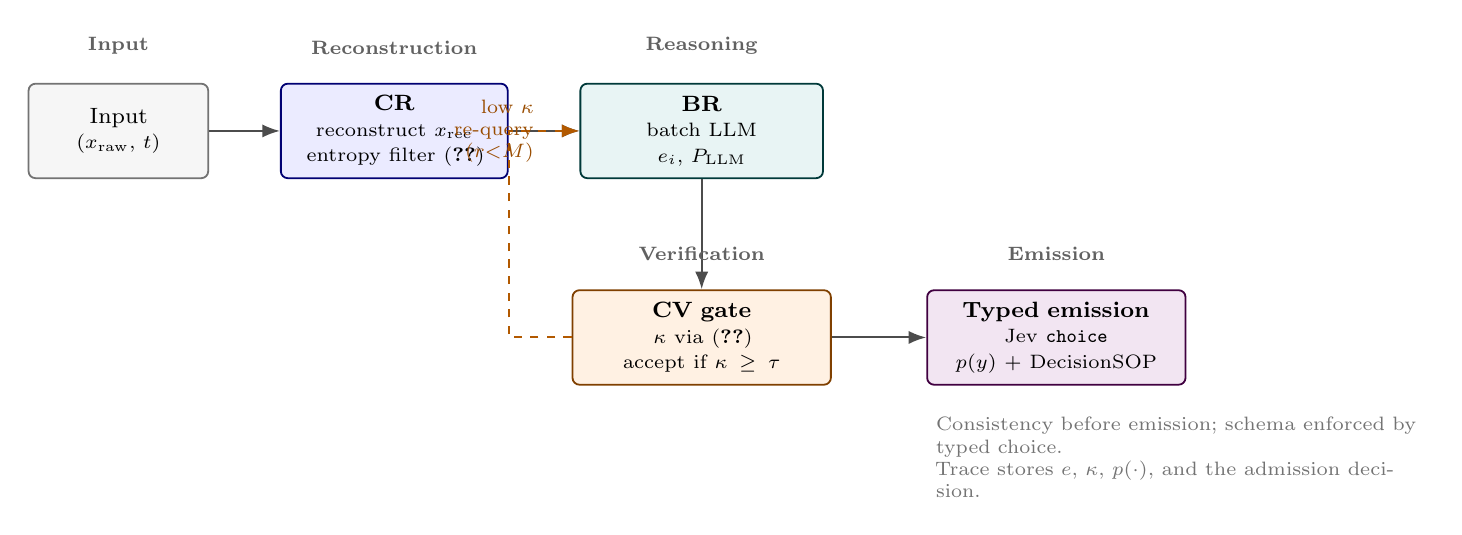
\begin{tikzpicture}[
  font=\footnotesize,
  >=Latex,
  box/.style={draw, rounded corners=2.5pt, align=center, inner sep=4pt,
    minimum height=12mm, line width=0.65pt},
  inbox/.style={box, fill=black!3.5, draw=black!55, text width=20mm},
  crbox/.style={box, fill=blue!8, draw=blue!45!black, text width=26mm},
  brbox/.style={box, fill=teal!9, draw=teal!45!black, text width=28mm},
  cvbox/.style={box, fill=orange!11, draw=orange!50!black, text width=30mm},
  outbox/.style={box, fill=violet!10, draw=violet!50!black, text width=30mm},
  arr/.style={->, line width=0.75pt, draw=black!70},
  lab/.style={font=\scriptsize\bfseries, text=black!62},
  note/.style={font=\scriptsize, align=left, text=black!55},
  pane/.style={draw=black!25, rounded corners=3pt, inner sep=5pt, fill=black!1.5}
]
  % top row
  \node[inbox] (in) {Input\\[-0.4pt]{\scriptsize $(x_{\mathrm{raw}},\,t)$}};
  \node[crbox, right=9mm of in] (cr) {\textbf{CR}\\[-0.3pt]{\scriptsize reconstruct $x_{\mathrm{rec}}$}\\[-0.3pt]{\scriptsize entropy filter~\eqref{eq:se}}};
  \node[brbox, right=9mm of cr] (br) {\textbf{BR}\\[-0.3pt]{\scriptsize batch LLM}\\[-0.3pt]{\scriptsize $e_i,\,P_{\mathrm{LLM}}$}};

  % bottom row
  \node[cvbox, below=14mm of br] (cv) {\textbf{CV gate}\\[-0.3pt]{\scriptsize $\kappa$ via~\eqref{eq:kappa}}\\[-0.3pt]{\scriptsize accept if $\kappa\ge\tau$}};
  \node[outbox, right=12mm of cv] (out) {\textbf{Typed emission}\\[-0.3pt]{\scriptsize Jev \texttt{choice}}\\[-0.3pt]{\scriptsize $p(y)$ + DecisionSOP}};

  \draw[arr] (in) -- (cr);
  \draw[arr] (cr) -- (br);
  \draw[arr] (br) -- (cv);
  \draw[arr] (cv) -- (out);

  % re-query loop
  \draw[arr, dashed, draw=orange!70!black] (cv.west) -- ++(-8mm,0) |- node[pos=0.75, left, font=\scriptsize, text=orange!60!black, align=right]{low $\kappa$\\re-query\\($r{<}M$)} (br.west);

  \node[lab, above=2.4mm of in] {Input};
  \node[lab, above=2.4mm of cr] {Reconstruction};
  \node[lab, above=2.4mm of br] {Reasoning};
  \node[lab, above=2.4mm of cv] {Verification};
  \node[lab, above=2.4mm of out] {Emission};

  \node[note, below=2.8mm of out.south west, anchor=north west, text width=62mm]{%
    Consistency before emission; schema enforced by typed choice.\\
    Trace stores $e$, $\kappa$, $p(\cdot)$, and the admission decision.};
\end{tikzpicture}}
\caption{StanceJEV system path (academic overview).
An input pair $(x,t)$ is reconstructed (CR), reasoned over in batch (BR), and scored by a consistency gate
(CV).
High-$\kappa$ items proceed immediately; low-$\kappa$ items re-query while $r{<}M$ or aggregate when multiple
rounds exist.
Typed Jev emission returns $p(y)$ and a DecisionSOP trace with $\hat{y}\in\mathcal{Y}$ by construction.}
\label{fig:pipeline}
\end{figure}

%==============================================================================
\section{Experimental Setup}
\label{sec:setup}
%==============================================================================

\paragraph{Datasets.}
SemEval-2016 Task~6 Subtask~A \cite{mohammad2016semeval} contributes the official test split of 1{,}249
labelled tweets over five targets (Atheism, Climate Change is a Real Concern, Feminist Movement, Hillary
Clinton, Legalization of Abortion).
Reported SemEval numbers are zero-shot \emph{inference} on that test split: no SemEval training tweets,
demonstrations drawn from train, or target-specific fine-tuning~/~supervision are used.
VAST \cite{allaway2020vast} contributes 1{,}460 official zero-shot test pairs ($\texttt{seen?}{=}0$) spanning
hundreds of topics, matching the CoVer zero-shot protocol \cite{yan2025cover}.
P-Stance \cite{li2021pstance} is a related political Twitter suite outside the primary tables of this study.

\paragraph{Backbones and protocol.}
Batch reasoning uses Xiaomi \texttt{mimo-v2.6-flash} via the OpenAI-compatible endpoint at
\texttt{api.xiaomimimo.com} (temperature $0.0$).
Typed decisions use the OpenRouter Decisions API with \texttt{typesafe/jev-1.13}.
The consistency verifier is a \emph{local} lexicon~/~heuristic scorer (no remote model): Jensen--Shannon
divergence is computed in base-$2$ bits on the three-label simplex, with mixture weight $\lambda{=}0.35$,
accept threshold $\tau{=}0.55$, and round budget $M{=}1$; BR batch size is $4$.
Context reconstruction in the reported SJ-1 runs is keep-all (no remote embedder;
\texttt{use\_embed\_filter}${}={}$\texttt{False}); optional knowledge is attached only when a knowledge field
is present (empty on these suites).
$Q_{\mathrm{AVG}}$ counts \emph{remote} LLM~/~decision API calls only.
Local consistency verification and keep-all CR do not add remote queries.
Under $M{=}1$ each item therefore costs one BR call plus one Jev decision call, hence
$Q_{\mathrm{AVG}}{=}2.0$; multi-round aggregation is inactive, while $\kappa$ is still computed and logged
for every prediction.
No random seed is set for the remote APIs beyond temperature $0.0$; the local verifier is deterministic given
its inputs.
We report $F_{\mathrm{AVG}}$ (SemEval), $F_{\mathrm{macro3}}$ (VAST), per-class F1, accuracy, schema-valid
rate, mean $\max_y p(y)$, mean $\kappa$, and distributional analyses over the typed prediction traces.

\paragraph{Implementation notes.}
Predictions are written as JSONL DecisionSOP-style records containing $\hat{y}$, $p(\cdot)$, $\kappa$,
explanation text, reconstructed input, and backend metadata; exact prompts and outputs are recoverable from
those traces.
All metrics below are recomputed from the records joined to gold labels; no free-form parse step enters the
scoring path.
Gold distributions differ across suites: SemEval test is Against-heavy ($715$ Against / $304$ Favor /
$230$ None), while VAST zero-shot is nearly balanced ($490$ / $451$ / $519$).
Predicted margins track these regimes without leaving $\mathcal{Y}$ (SemEval predictions:
$567$ Against / $379$ Favor / $303$ None; VAST: $477$ / $484$ / $499$).
Every item used exactly two \emph{remote} queries under this protocol ($Q_{\mathrm{AVG}}{=}2.0$).

%==============================================================================
\section{Results}
\label{sec:results}
%==============================================================================

\subsection{Zero-shot typed accuracy}
Table~\ref{tab:overall} reports overall zero-shot performance.
Every label is emitted through the typed choice, so accuracy is measured without a free-form parse step.
Schema validity is $100\%$ on both suites by construction of Definition~\ref{def:typedstance}
($N{=}2{,}709$ typed emissions).

\begin{table}[H]
\centering
\small
\begin{tabular}{lrrrrr}
\toprule
Dataset & $n$ & Primary & Acc. & Schema & $Q_{\mathrm{AVG}}$ \\
\midrule
SemEval-2016 Task~A & 1249 & $0.785$ ($F_{\mathrm{AVG}}$) & $0.762$ & $100\%$ & $2.0$ \\
VAST zero-shot & 1460 & $0.833$ ($F_{\mathrm{macro3}}$) & $0.834$ & $100\%$ & $2.0$ \\
\bottomrule
\end{tabular}
\caption{Zero-shot StanceJEV on SemEval-2016 Task~A and VAST.
SemEval uses Favor~/~Against macro-F1 ($F_{\mathrm{AVG}}$); VAST uses three-label mean F1 ($F_{\mathrm{macro3}}$).
Schema is the fraction of predictions in $\{\texttt{Favor},\texttt{Against},\texttt{None}\}$.}
\label{tab:overall}
\end{table}

On SemEval, Favor F1 ${=}0.764$ and Against F1 ${=}0.807$ (None F1 ${=}0.653$).
Table~\ref{tab:sem16-target} breaks results down by target: Hillary Clinton is strongest
($F_{\mathrm{AVG}}{=}0.833$) and Legalization of Abortion hardest ($0.686$).
On VAST zero-shot, per-class F1 is Favor ${0.802}$, Against ${0.796}$, None ${0.900}$.
Table~\ref{tab:perclass} reports precision, recall, and F1 for each label; Table~\ref{tab:confusion}
gives the full confusion counts used to derive those scores.

\begin{table}[H]
\centering
\small
\begin{tabular}{llrrr}
\toprule
Dataset & Label & Prec. & Rec. & F1 \\
\midrule
\multirow{3}{*}{SemEval-2016}
 & Favor & $0.689$ & $0.859$ & $0.764$ \\
 & Against & $0.912$ & $0.723$ & $0.807$ \\
 & None & $0.574$ & $0.757$ & $0.653$ \\
\midrule
\multirow{3}{*}{VAST zero-shot}
 & Favor & $0.775$ & $0.831$ & $0.802$ \\
 & Against & $0.807$ & $0.786$ & $0.796$ \\
 & None & $0.918$ & $0.882$ & $0.900$ \\
\bottomrule
\end{tabular}
\caption{Per-class precision, recall, and F1 under typed StanceJEV (computed from prediction traces).}
\label{tab:perclass}
\end{table}

\begin{table}[H]
\centering
\small
\begin{tabular}{llrrr}
\toprule
& & \multicolumn{3}{c}{Predicted} \\
\cmidrule(lr){3-5}
Dataset & Gold & Favor & Against & None \\
\midrule
\multirow{3}{*}{SemEval-2016}
 & Favor & 261 & 15 & 28 \\
 & Against & 97 & 517 & 101 \\
 & None & 21 & 35 & 174 \\
\midrule
\multirow{3}{*}{VAST zero-shot}
 & Favor & 375 & 57 & 19 \\
 & Against & 83 & 385 & 22 \\
 & None & 26 & 35 & 458 \\
\bottomrule
\end{tabular}
\caption{Confusion counts for typed predictions versus gold labels.}
\label{tab:confusion}
\end{table}

\begin{table}[H]
\centering
\small
\begin{tabular}{lrrrr}
\toprule
Target & $n$ & $F_{\mathrm{AVG}}$ & Acc. & None F1 \\
\midrule
Atheism & 220 & $0.760$ & $0.759$ & $0.585$ \\
Climate Change is a Real Concern & 169 & $0.815$ & $0.805$ & $0.634$ \\
Feminist Movement & 285 & $0.759$ & $0.761$ & $0.686$ \\
Hillary Clinton & 295 & $0.833$ & $0.824$ & $0.743$ \\
Legalization of Abortion & 280 & $0.686$ & $0.675$ & $0.583$ \\
\midrule
Macro (SemEval test) & 1249 & $0.785$ & $0.762$ & $0.653$ \\
\bottomrule
\end{tabular}
\caption{SemEval-2016 Task~A per-target breakdown under the typed StanceJEV path.}
\label{tab:sem16-target}
\end{table}

\subsection{Typed fidelity}
Table~\ref{tab:fidelity} reports schema rate together with concentration of decision mass and mean
consistency.
Mean $\max_y p(y)$ is $0.868$ on SemEval and $0.907$ on VAST; mean $\kappa$ is $0.767$ and $0.784$,
respectively.
Peak probability concentrates without a post-hoc parser; $\kappa$ summarizes batch--verifier agreement under
$M{=}1$.
Median $\kappa$ is $0.829$ (SemEval) and $0.867$ (VAST); the $10$th--$90$th percentiles span roughly
$[0.49,0.96]$ and $[0.51,0.96]$.

\begin{table}[H]
\centering
\small
\begin{tabular}{lrrr}
\toprule
Dataset & Schema-valid & mean $\max_y p(y)$ & mean $\kappa$ \\
\midrule
SemEval-2016 Task~A & $100\%$ & $0.868$ & $0.767$ \\
VAST zero-shot & $100\%$ & $0.907$ & $0.784$ \\
\bottomrule
\end{tabular}
\caption{Typed-decision fidelity: schema-valid rate, mean peak probability, and mean consistency $\kappa$.}
\label{tab:fidelity}
\end{table}

\subsection{Consistency and confidence analysis}
\label{sec:analysis}
Tables~\ref{tab:kappa-bins} and~\ref{tab:maxp-bins} stratify accuracy by $\kappa$ and by typed peak
probability, computed directly from the prediction JSONL joined to gold labels.

\begin{table}[H]
\centering
\small
\begin{tabular}{lrrrrrr}
\toprule
& \multicolumn{3}{c}{SemEval-2016} & \multicolumn{3}{c}{VAST zero-shot} \\
\cmidrule(lr){2-4}\cmidrule(lr){5-7}
$\kappa$ bin & $n$ & Acc. & mean $\kappa$ & $n$ & Acc. & mean $\kappa$ \\
\midrule
$[0,0.55)$ & 178 & $0.798$ & $0.428$ & 205 & $0.912$ & $0.439$ \\
$[0.55,0.70)$ & 259 & $0.822$ & $0.615$ & 201 & $0.836$ & $0.624$ \\
$[0.70,0.85)$ & 212 & $0.656$ & $0.775$ & 291 & $0.790$ & $0.770$ \\
$[0.85,1]$ & 600 & $0.763$ & $0.930$ & 763 & $0.830$ & $0.925$ \\
\bottomrule
\end{tabular}
\caption{Accuracy stratified by consistency $\kappa$ under $M{=}1$.
$\kappa$ measures agreement between $P_{\mathrm{LLM}}$ and the verifier; it is not assumed to be a
calibrated correctness score.}
\label{tab:kappa-bins}
\end{table}

\begin{table}[H]
\centering
\small
\begin{tabular}{lrrrrrr}
\toprule
& \multicolumn{3}{c}{SemEval-2016} & \multicolumn{3}{c}{VAST zero-shot} \\
\cmidrule(lr){2-4}\cmidrule(lr){5-7}
$\max_y p(y)$ bin & $n$ & Acc. & mean $\max p$ & $n$ & Acc. & mean $\max p$ \\
\midrule
$[0,0.70)$ & 212 & $0.561$ & $0.567$ & 185 & $0.465$ & $0.565$ \\
$[0.70,0.85)$ & 195 & $0.574$ & $0.776$ & 150 & $0.680$ & $0.772$ \\
$[0.85,0.95)$ & 226 & $0.743$ & $0.900$ & 151 & $0.735$ & $0.902$ \\
$[0.95,1]$ & 616 & $0.898$ & $0.988$ & 974 & $0.944$ & $0.993$ \\
\bottomrule
\end{tabular}
\caption{Accuracy stratified by typed peak probability $\max_y p(y)$.
High peak mass concentrates on correct items on both suites.}
\label{tab:maxp-bins}
\end{table}

Two patterns are visible.
First, accuracy rises monotonically across these $\max_y p(y)$ bins: on SemEval, from
$0.561$ in $[0,0.70)$ to $0.898$ in $[0.95,1]$; on VAST the corresponding rise is $0.465\rightarrow 0.944$.
Mean $\max_y p(y)$ is $0.897$ on correct SemEval items versus $0.774$ on errors ($0.938$ vs.\ $0.753$ on
VAST).
Second, $\kappa$ under $M{=}1$ characterizes batch--verifier agreement rather than monotonic correctness:
low-$\kappa$ bins are not the least accurate strata in Table~\ref{tab:kappa-bins}.
This separation is useful for monitoring design---$\kappa$ and $\max_y p(y)$ are distinct axes on the
DecisionSOP surface, in the spirit of keeping evaluation axes separable
\cite{souly2024strongreject,yan2025confusion}.

LLM argmax labels agree with the typed emission on $82.6\%$ of SemEval items and $88.4\%$ of VAST items,
indicating that the typed endpoint usually consolidates the batch likelihood but is not a trivial copy of
$P_{\mathrm{LLM}}$.

\subsection{Error structure and qualitative examples}
\label{sec:qual}
On SemEval, the dominant confusions are Against$\rightarrow$None ($101$) and Against$\rightarrow$Favor
($97$), with fewer Favor$\rightarrow$None ($28$) and Favor$\rightarrow$Against ($15$) swaps.
On VAST, Favor$\leftrightarrow$Against flips dominate ($57{+}83$), while None remains comparatively reliable
(None F1 $0.900$).
These patterns align with target difficulty in Table~\ref{tab:sem16-target}: contested social targets
(abortion, feminism) admit polarity reversals when sarcasm or quote attribution is ambiguous.

Table~\ref{tab:cases} lists short illustrative cases (text truncated) drawn from the typed traces.
High-$\kappa$ correct None decisions often correspond to inputs that never mention the target; high-$\kappa$
errors include polarity reversals on sarcastic or multi-entity posts; low-$\kappa$ items can still be correct
when the typed peak mass is decisive---consistent with treating $\kappa$ as an agreement signal rather than a
substitute for $p(y)$.

\begin{table}[H]
\centering
\scriptsize
\begin{tabular}{p{1.6cm}p{1.5cm}ccp{4.6cm}p{3.4cm}}
\toprule
Suite / id & Target & Gold & Pred & Truncated input & Note \\
\midrule
SE 10750 & Hillary Clinton & None & None & ``\ldots WHAT DID HE SAY? \ldots \#OBAMA \#ISIS'' & High $\kappa$; target unmentioned \\
SE 10438 & Feminist Movement & Against & Favor & ``\ldots women being meninists/MRAs? \ldots'' & High $\kappa$; polarity reverse \\
SE 10930 & Hillary Clinton & Against & Against & ``Hillarity claims no subpoenas\ldots'' & Low $\kappa$; typed Against correct \\
VA 23211 & printer & None & None & Urban pollution / bike-lane comment & Low $\kappa$; unrelated target \\
\bottomrule
\end{tabular}
\caption{Illustrative typed traces (inputs truncated).
Cases show schema-bound labels under both high- and low-$\kappa$ regimes.}
\label{tab:cases}
\end{table}

%==============================================================================
\section{Discussion}
\label{sec:discussion}
%==============================================================================

\subsection{Implication of the typed terminal contract}
Free-form stance pipelines optimize a predictive score and then rely on parsers to recover $\mathcal{Y}$.
StanceJEV inverts that order: $\mathcal{Y}$ is the action set from the start, so schema fidelity is a property
of the interface rather than a cleanup step.
The measured $100\%$ schema-valid rate on 2{,}709 test items is the empirical counterpart of that design.
Accuracy remains necessary---$F_{\mathrm{AVG}}{=}0.785$ and $F_{\mathrm{macro3}}{=}0.833$ show that the typed
path is usable for zero-shot monitoring---but accuracy alone would still leave the decision interface
unsolved.

For product and agent consumers, the DecisionSOP surface supplies three separable quantities:
the label $\hat{y}\in\mathcal{Y}$, the probability vector $p(\cdot)$, and the admission signal $\kappa$.
Tables~\ref{tab:kappa-bins}--\ref{tab:maxp-bins} show why separation matters: peak typed probability tracks
correctness closely, while $\kappa$ reports a different property of the batch--verifier pair.
Operators can threshold on $\max_y p(y)$ for routing confidence and retain $\kappa$ for audit of explanation
coherence, without conflating the two.

This framing also clarifies what accuracy-only papers leave implicit.
A system can raise $F_{\mathrm{AVG}}$ while still forcing every deployer to invent a parser; conversely, a typed
system with slightly lower free-form-comparable accuracy can be preferable when schema failures are
operationally unacceptable.
StanceJEV's measured universal schema validity on both suites makes that trade-off explicit rather than
hidden in evaluation scripts.
Confusion structure (Table~\ref{tab:confusion}) further shows where human review should concentrate:
Against$\rightarrow$None and Against$\rightarrow$Favor on SemEval, and Favor$\leftrightarrow$Against flips on
VAST, rather than schema repair.

\subsection{Relation to collaborative SLLM pipelines}
CoVer demonstrates that small--large consistency verification can raise zero-shot stance accuracy at low query
cost \cite{yan2025cover}.
StanceJEV does not replace that collaboration; it changes where the collaboration terminates.
CR~/~BR~/~CV remain the path that constructs and admits state $s$; the typed Jev choice is the contract that
makes $s$ consumable by code.
In that sense the paper's scientific claim is about the \emph{terminal interface} of stance monitoring, not
about displacing collaborative reasoning as a research line.
A useful mental model is a layered stack: collaborative SLLM reasoning proposes and checks evidence; the typed
choice commits an action in $\mathcal{Y}$; DecisionSOP persists the commitment for downstream code.
Removing the top layer returns the free-form monitoring problem; removing the middle layer returns an unchecked
typed emission; removing the bottom layer returns an un-auditable decision.
Companion security work on the same typed interface studies adversarial probability shifts inside closed
action sets \cite{wu2026decisionhijacking,yan2025benign,yan2026searchattack}; monitoring and security share
the contract while asking different questions of it.

\subsection{Scope and open questions}
Results use one primary backbone pair (\texttt{mimo-v2.6-flash} + \texttt{typesafe/jev-1.13}) at fixed
$Q_{\mathrm{AVG}}{=}2.0$ and $M{=}1$.
Several scientific questions follow directly from the present evidence without requiring a change of problem
definition.
How does multi-round aggregation under $M{>}1$ reshape the joint distribution of $(\kappa,\max_y p(y))$ on
the same typed surface?
When do free-form and typed endpoints diverge on identical batch evidence, and which divergence modes are
schema failures versus polarity failures?
How should retrieved knowledge be gated before it enters $s$, given search-augmented misuse risks
\cite{yan2026searchattack,yan2025poisonswarm}?
Does target-conditioned calibration of $\tau$ reduce Against$\rightarrow$None leakage on contested SemEval
targets without harming VAST None reliability?
Domain retuning of $\tau$ and richer CR on rare VAST topics are natural extensions of the same evaluation
surface.
These questions keep the scientific object fixed---typed stance with a consistency path---while varying the
evidence that the object must explain.
Adaptive injection on the typed interface is studied in companion security work
\cite{wu2026decisionhijacking,debenedetti2024agentdojo}.
Raw social-media text is processed under dataset licenses and is not redistributed with this draft.

%==============================================================================
\section{Conclusion}
\label{sec:conclusion}
%==============================================================================

Zero-shot stance for monitoring is a closed decision problem.
Existing LLM and collaborative pipelines improve free-form accuracy and cost while leaving the terminal
interface open-ended.
StanceJEV formulates the task as a typed probabilistic choice over $\mathcal{Y}$, places a CoVer-style
consistency path before emission, and terminates in a DecisionSOP contract.
On SemEval-2016 Task~A the typed path reaches $F_{\mathrm{AVG}}{=}0.785$ at $Q_{\mathrm{AVG}}{=}2.0$ with
universal schema validity; on VAST zero-shot it reaches $F_{\mathrm{macro3}}{=}0.833$ under the same
configuration.
Typed peak probability concentrates on correct items; consistency $\kappa$ remains an auditable
batch--verifier agreement signal under a single-round budget.
Stance is already a closed action set---evaluating only free-form accuracy leaves the decision interface
unsolved.

\section*{Ethical Considerations}
Stance systems can amplify political or demographic skew if deployed without audit \cite{li2024factual}.
Schema-bound labels and DecisionSOP traces support review of both the predicted class and the admission
decision ($\kappa$).
Search-augmented misuse risks noted by prior work apply when retrieval is attached
\cite{yan2026searchattack}; operators should gate external content before it enters state $s$.
Distributed synthesis threats further motivate logging typed decisions at scale rather than free-form
generations alone \cite{yan2025poisonswarm}.
Datasets must be used under their licenses; raw social-media text is not redistributed with this draft.
Illustrative examples in Table~\ref{tab:cases} are truncated and are not a release of the underlying corpora.

\begingroup
\small
\bibliographystyle{plain}
\bibliography{references}
\endgroup
\end{document}
